\documentclass{article}\usepackage[]{graphicx}\usepackage[]{color}
%% maxwidth is the original width if it is less than linewidth
%% otherwise use linewidth (to make sure the graphics do not exceed the margin)
\makeatletter
\def\maxwidth{ %
  \ifdim\Gin@nat@width>\linewidth
    \linewidth
  \else
    \Gin@nat@width
  \fi
}
\makeatother

\definecolor{fgcolor}{rgb}{0.345, 0.345, 0.345}
\newcommand{\hlnum}[1]{\textcolor[rgb]{0.686,0.059,0.569}{#1}}%
\newcommand{\hlstr}[1]{\textcolor[rgb]{0.192,0.494,0.8}{#1}}%
\newcommand{\hlcom}[1]{\textcolor[rgb]{0.678,0.584,0.686}{\textit{#1}}}%
\newcommand{\hlopt}[1]{\textcolor[rgb]{0,0,0}{#1}}%
\newcommand{\hlstd}[1]{\textcolor[rgb]{0.345,0.345,0.345}{#1}}%
\newcommand{\hlkwa}[1]{\textcolor[rgb]{0.161,0.373,0.58}{\textbf{#1}}}%
\newcommand{\hlkwb}[1]{\textcolor[rgb]{0.69,0.353,0.396}{#1}}%
\newcommand{\hlkwc}[1]{\textcolor[rgb]{0.333,0.667,0.333}{#1}}%
\newcommand{\hlkwd}[1]{\textcolor[rgb]{0.737,0.353,0.396}{\textbf{#1}}}%

\usepackage{framed}
\makeatletter
\newenvironment{kframe}{%
 \def\at@end@of@kframe{}%
 \ifinner\ifhmode%
  \def\at@end@of@kframe{\end{minipage}}%
  \begin{minipage}{\columnwidth}%
 \fi\fi%
 \def\FrameCommand##1{\hskip\@totalleftmargin \hskip-\fboxsep
 \colorbox{shadecolor}{##1}\hskip-\fboxsep
     % There is no \\@totalrightmargin, so:
     \hskip-\linewidth \hskip-\@totalleftmargin \hskip\columnwidth}%
 \MakeFramed {\advance\hsize-\width
   \@totalleftmargin\z@ \linewidth\hsize
   \@setminipage}}%
 {\par\unskip\endMakeFramed%
 \at@end@of@kframe}
\makeatother

\definecolor{shadecolor}{rgb}{.97, .97, .97}
\definecolor{messagecolor}{rgb}{0, 0, 0}
\definecolor{warningcolor}{rgb}{1, 0, 1}
\definecolor{errorcolor}{rgb}{1, 0, 0}
\newenvironment{knitrout}{}{} % an empty environment to be redefined in TeX

\usepackage{alltt}
\input{c:/aaaWork/zGnrlLatex/GnrlPreamble}
\hypersetup{pdftitle = R Workshop Install}
\input{c:/aaaWork/zGnrlLatex/JustRPreamble}
\setcounter{secnumdepth}{0}  % have unnumbered sections appear in TOC
\IfFileExists{upquote.sty}{\usepackage{upquote}}{}
\begin{document}


\section{Preparing RStudio}
\begin{enumerate}
  \item Open RStudio.

  \item Select the ``Tools'' menu and then the ``Global Options'' submenu.  In the ensuing dialog box select the ``General'' icon on the left (this should already be selected).
\begin{center}
  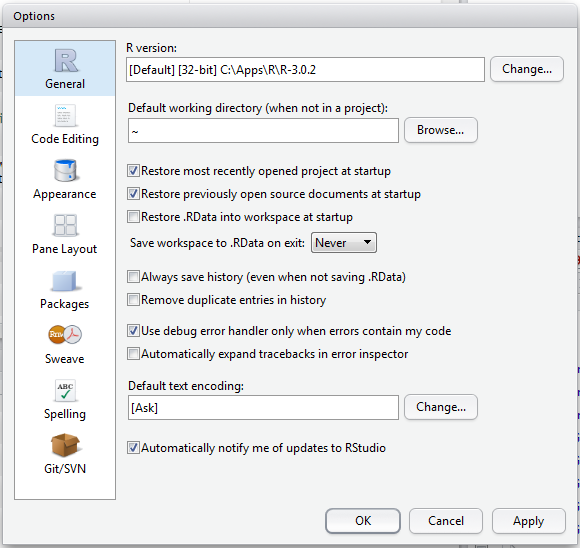
\includegraphics[width=3in]{Figs/RStudio_Prep_OptionsGeneral.png}
\end{center}
  \begin{itemize}
    \item Depending on your installation, the R version should read ``[Default][32-bit]'' followed by the path to the R program (as shown in the dialog box above).  If you installed the 64-bit version of R then select the ``Change...'' button and then select ``use your machine's default version of R64 (64-bit)''.
    \item You can either leave the other selections at their defaults or change them as you see fit (my preferences are shown in the dialog box above).  However, I strongly urge you to un-select ``Restore .RData into workspace at startup''.
  \end{itemize}

  \item Select the ``Packages'' icon in the ``options'' dialog box opened above.  It is useful to set a CRAN mirror in this dialog box.  I prefer the ``0-Cloud - Rstudio ...'' option but you may want to choose a location nearer to you (through the ``change'' button).  All other options can remain at their defaults.
\begin{center}
  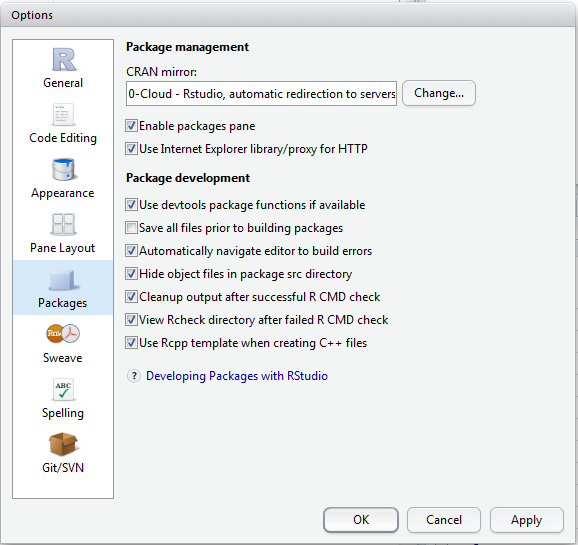
\includegraphics[width=3in]{Figs/RStudio_Prep_OptionsCRAN.png}
\end{center}

  \newpage
\item Select the ``Code Editing'' icon in the ``Options'' dialog box opened above.  I suggest, in addition to the default selections, selecting the ``Highlight selected line'', ``Show margin'', and ``Show syntax highlighting in console input.''
\begin{center}
  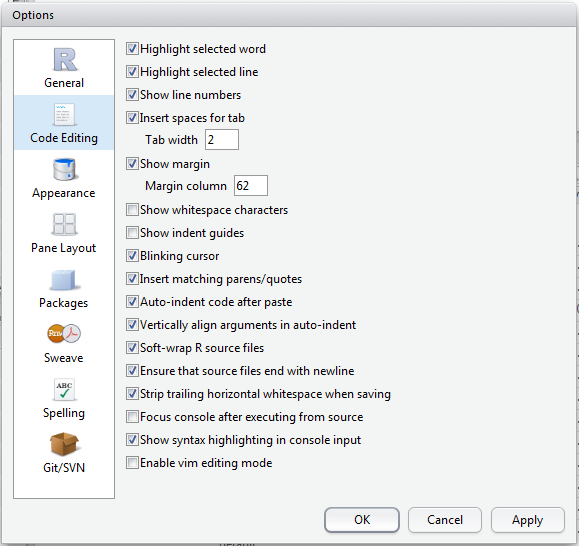
\includegraphics[width=3in]{Figs/RStudio_Prep_OptionsCodeEditing.png}
\end{center}

  \item No other options need to be set for our purposes.  Press ``OK.''
\end{enumerate}


\newpage
\section{Installing R Packages from CRAN}
R can be extended with external packages.  In this workshop, we will use several packages that are distributed via CRAN.  These packages are installed by following these directions.
\begin{enumerate}
  \item Open RStudio (if not already open).

  \item Select the ``Packages'' tab in the lower-right pane and then the ``Install'' button/graphic.
\begin{center}
  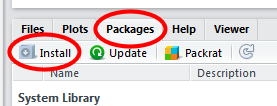
\includegraphics[width=2in]{Figs/RStudio_Prep_InstallPkgs_Icons.png}
\end{center}

  \item Type the name of the packages to be installed in the ``Packages (separate multiple packages with a space or comma):'' box.  Make sure the ``Install dependencies'' option is checked.  For this workshop we will need the \textit{dplyr}, \textit{magrittr}, and \textit{plotrix} packages.
\begin{center}
  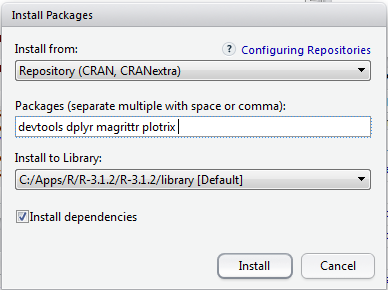
\includegraphics[width=3in]{Figs/RStudio_Prep_InstallPkgs_Choose.png}
\end{center}
  \item Press ``Install''.  RStudio should now install these packages plus all packages that these depend on.  This may take several minutes and you should see several ``package 'xxx' successfully unpacked and MD5 sums checked'' messages.
\end{enumerate}


\newpage
\section{Installing FSA and fishWiDNR from RForge.net}
The \R{FSA} and \R{fishWiDNR} packages are special purpose packages that we will use in this workshop that have not been officially released on CRAN.  These packages are available in RForge.net repositories and can be installed following these directions.
\begin{enumerate}
  \item Open RStudio (if not already open).

  \item Open a new R script pane by selecting the ``New'' icon to the far left on the RStudio toolbar (
\includegraphics[scale=0.8]{Figs/RStudio_Icon_New.png}) and choosing ``R script'' in the ensuing list (alternatively, use the \verb+<CTRL>+ + \verb+<Shift>+ + \verb+N+ keystrokes or select the \verb+File..+ \verb+New..+ \verb+R Script+ menu items).  This will open a blank script in the upper-left pane of the RStudio window (below the toolbar, above the ``Console'' pane).
\begin{center}
  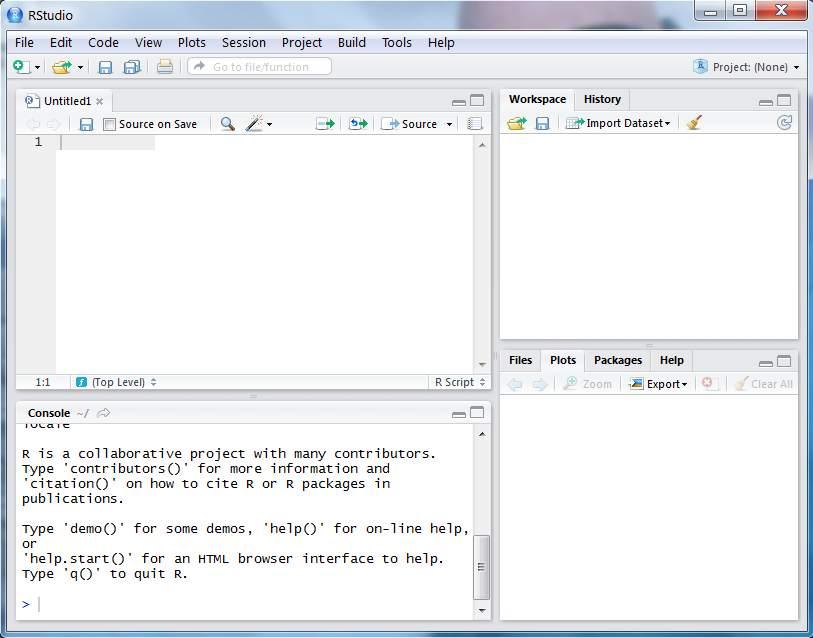
\includegraphics[width=4.5in]{Figs/RStudio_NewScript.png}
\end{center}

  \item In the R script pane, type the following code exactly:.
\begin{knitrout}
\definecolor{shadecolor}{rgb}{0.969, 0.969, 0.969}\color{fgcolor}\begin{kframe}
\begin{alltt}
\hlkwd{source}\hlstd{(}\hlstr{"http://www.rforge.net/fishWiDNR/InstallfishWiDNR.R"}\hlstd{)}
\end{alltt}
\end{kframe}
\end{knitrout}
\vspace{12pt}
  \item With the cursor on the line just typed, press the ``Run'' button (
\includegraphics[scale=0.8]{Figs/RStudio_Icon_Run.png}) near the far right of the ``R Script'' pane toolbar (alternatively press \verb+<CTRL>+ + \verb+<Enter>+).  This will ``send'' the R command to the Console pane.  RStudio should now download  the \R{FishWiDNR} and \R{FSA} packages and all associated dependencies.  This may take several minutes with a finish noted by an R prompt (a ``greater than'') symbol in the Console pane.
  \item Start a new line in the R script pane and type \R{library(fishWiDNR)}.  With the cursor on the line, press the ``Run'' button.  Start a new line in the R script pane and type \R{library(FSA)}.  With the cursor on the line, press the ``Run'' button.  The end of your Console pane should look like that below (the version number may be different).  If you received an error after running \R{library(FSA)}, then see the next section.
\begin{center}
  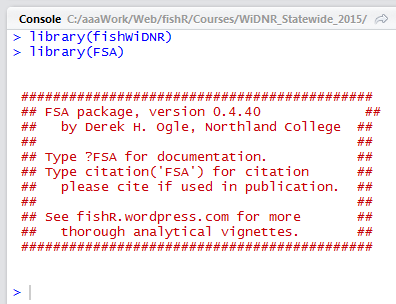
\includegraphics[width=2.5in]{Figs/RStudio_Prep_FSA.png}
\end{center}

  \item Start a new line in the R script pane and type \R{?FSA}.  With the cursor on the line, press the ``Run'' button.  A help page that looks like that shown below should appear in the ``Help'' pane in the lower-right corner of the RStudio window.  If this help page appears, then the installation is complete and correct.  If the help page does not appear, then see the next section.
\begin{center}
  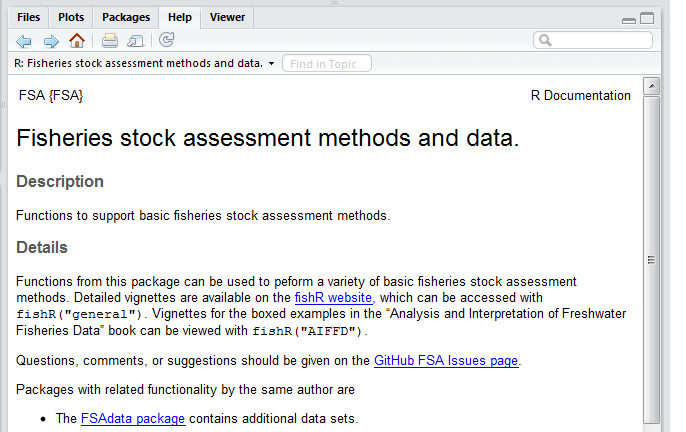
\includegraphics[width=3.5in]{Figs/RStudio_Prep_FSAHelp.png}
\end{center}
\end{enumerate}

\section{Troubleshooting the Installation of the FSA Package.}
The \R{FSA} package is not yet an official R package and, thus, the installation is non-standard.  My experience suggests that about 10\% of installations on Windows machines will result in some sort of error that will cause the \R{FSA} package to not be installed properly.  The primary cause of this problem is that one or more of the official R packages that the \R{FSA} package depends on was not installed properly.  You can identify this problem by looking closely at the output following the running of the \R{source()} line above.  For example, two typical errors are shown below.

\begin{center}
  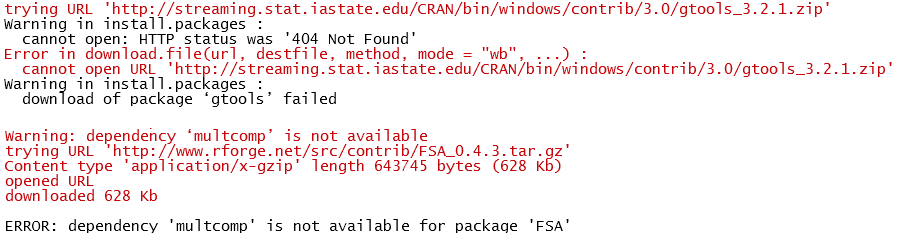
\includegraphics[width=5in]{Figs/RStudio_Prep_FSAInstallErrors.png}
\end{center}

The first error above indicates that the \R{gtools} package was not installed and the second error shows that the \R{multcomp} package was not installed.  If these specific errors occurred, then one would need to ``manually' install these packages as shown in the previous section.

\section{Questions?}
If you have any questions please contact Derek Ogle at \href{mailto:dogle@northland.edu}{dogle@northland.edu}.  Please make sure to include your operating systems (Windows PC, Mac, Linux/Unix) when contacting me with questions.

A small percentage of users will have trouble automatically installing the FSA package (and the packages that it depends on) to their computer (see the previous section).  If you are in this small group, then send me a message indicating your operating system and pasting the ``error results'' from the Console pane (lower-left pane in RStudio) into the e-mail message.

\end{document}
